
\textit{Results from this chapter are preliminary and have not been reviewed yet by the LIGO Scientific Collaboration.}
%\newline

        \section{Directed TwoSpect}
        \label{directed}

TwoSpect performed aptly in Chapter~\ref{chap5}'s Mock Data Challenge, which warrants using the program to analyze the best existing GW data.
At the time of writing, the best consistent stretch of data remains Science Run 6 (S6) taken from 2009 July 09 to 2010 October 20 by LIGO Hanford Observatory (LHO) and LIGO Livingston Observatory (LLO).
Advanced LIGO (aLIGO) commissioning is already surpassing the sensitivity of S6 for short periods of time.
While early LIGO continuous wave (CW) searches used short science runs such as S2~\cite{AbbottScoX12007}, aLIGO data duration is for now too short for an analysis competitive with present upper limits, in particular the 2011 Radiometer~\cite{AbadieStoch2011} S5 high frequency results and 2014 TwoSpect~\cite{GoetzTwoSpectResults2014} S6 low frequency results.
The increased sensitivity anticipated from aLIGO Observing Run 1 (O1), which is planned to last several months in summer 2015, could yield interesting results, and the 9-month O3 is planned before the end of the decade.
Preliminary Scorpius X-1 broadband upper limits from S6 are presented in this chapter.

            %TwoSpect improvements myself (to do).

            \subsection{Targeted, directed and all-sky search sensitivity}
            \label{tradeoffs}

Several approaches exist toward a search for GW from known objects such as Scorpius X-1\footnote{Discovered by Riccardo Giacconi.}.
When seeking continuous GW, these methods are classified as all-sky, directed, or targeted, in order of increasing focus of the search.
More focused searches make sense as more prior information is known, such as sky location, neutron star frequency and binary system orbital parameters.
Additional information lets some CW searches refine, for instance, their template models of GW signals.
If the search is designed for minimal information, in particular if sky location is unknown, it is generally called an \textit{all-sky search}.
Some information -- such as a low-uncertainty sky-location, less than a square arcminute -- helps what are called \textit{directed searches} gain sensitivity.
Sources with comprehensively documented parameters, such as rotation frequency and spindown rate, lend themselves to \textit{targeted searches} that search over a very narrow range of parameters, \textit{e.g.,} putative GW phase and orientation angles.

TwoSpect was designed~\cite{GoetzThesis,GoetzTwoSpectMethods2011} as an all-sky search for unknown neutron stars.
The voluminous parameter space of that search, as described in Chapter~\ref{chap5}, prompted tradeoffs in sensitivity vs computational cost, in particular the limitation of test statistic calculation to only those outlier candidates that survived an incoherent harmonic sum stage. 
For objects with constrained sky location and NS parameters, thorough calculations of the $R$ test statistic become feasible.

For Scorpius X-1, many parameters are known (updated ephemerides were calculated in 2014 by Galloway~\cite{Galloway2014}), but critically, rotation frequency is not.
Sky location is known, and the period is $0.7873114 \pm 0.0000005$ days, \textit{i.e.,} $68023.70 \pm 0.04$ s with 1-$\sigma$ uncertainty\footnote{Access to a preliminary ephemeris in the MDC led us to use $P = 68023.8259 s$ in for searches in the MDC and S6; MDC simulations justify assuming that this variation has negligible impact on TwoSpect, which would only be able to discriminate between different periods around $68023 s$ at a resolution of about $40 s$ or greater, depending on Fourier transform coherence time.}.
The projected semimajor axis, $a \sin i$, is $1.44 \pm 0.18 s$ with 1-$\sigma$ uncertainty\footnote{Orbital parameters interpreted in correspondence between C. Messenger and D. Galloway.}.
Rotation frequency uncertainty drives the cost of the search.
While the Chakrabarty speed limit~\cite{Chakrabarty2003} and neutron star breakup limit limit $2\nu$, the GW emission frequency of an NS quadrupole, to $\mathcal{O}(2\textup{ to }3)$ kHz, the dominant high frequency limit $f_h$ is driven as much by the noise floor of the LIGO detectors.
This noise floor increases linearly with frequency and at 2 kHz is an order of magnitude worse than its most sensitive, about $2\times10^{-23}$ in dimensionless strain between 150 and 200 Hz.
Photon shot noise, that is, quantum vacuum fluctuations are the limiting noise source at those frequencies.
The low-frequency limit, $f_l$, is also driven by the noise floor of the detector, which becomes contaminated by seismic noise below about 40~Hz.

A search for Scorpius X-1 in S6 data should thus take place between about 40 and 2000 Hz. 
TwoSpect requires shortened Short Fourier Transforms (SFTs)~\cite{GoetzTwoSpectMethods2011} to fully capture the spectral power if a GW source has a high frequency or large $a \sin i$. 
This suggests dividing the main search: 40 to 360 Hz can be searched in 840-s coherence time SFTs and 360 to 2040 Hz in 360-s coherence time SFTs.
These sets constitute the primary search.
Although MDC and simulation experience suggests spectral power is lost only slowly as GW frequency exceeds optimal coherence time, we have also prepared 260 Hz to 360 Hz SFTs with 360-s coherence time and 1400 Hz to 2040 Hz SFTs with 300-s coherence time; these are most useful for high $a \sin i$ signal models.
These additional sets constitute the `overlap' search.
Calculating the number of templates in the primary search (the overlap search is smaller because of shorter coherence times) over these frequencies and $\pm 3 \sigma_{a \sin i}$, if analyzed in 0.1 Hz computational bands\footnote{0.1 Hz computational bands fit efficiently on cluster memory in under 2 GB of RAM; for convenience, templates are (redundantly) tested at both the lower \& upper bounds of the 0.1 Hz.} using Equation~\ref{N_template_simple},

\begin{equation}
N_\textup{template} = 2 (840.1)\left[1+ \frac{3360\pi}{68023.8} 400.1 \right](320) + 2 (360.1)\left[1+ \frac{1440\pi}{68023.8}2400.1\right](1680),
\label{S6_N_templates}
\end{equation}

\noindent or $3.392\times 10^7$ templates in 840-s SFTs and $1.9434\times 10^8$ templates in 360-s SFTs, per interferometer.
Searching both LHO's H1 interferometer and LLO's L1 interferometer, the grand total is $4.5652\times10^8$ templates.

Each of these templates takes between 0.3 and 3 s to run on late 2000s to early 2010s CPUs, depending on vector extensions (such as SSE) and clock speed.
Given approximately two thousand cores at a cluster such as the LIGO Data Grid at the California Institute of Technology and the LIGO observatories or Atlas at the Albert Einstein Institute in Hannover, Germany, a fully templated TwoSpect search for Scorpius X-1 in S6 data can be completed in roughly a month.
This has been carried out by the author and is the subject of the remainder of this chapter.
Because of the enhanced sensitivity and wider frequency range of the directed search, this analysis can improve on the TwoSpect all-sky limits by Goetz~\cite{GoetzTwoSpectResults2014} despite consuming much fewer computational resources (albeit for a single, promising source).

             %   Targeted (known object) vs directed (region)vs all-sky (everything).

            \subsection{Enhancements enabled by directed searching}
            \label{directed_enhancements}

Directed TwoSpect as used for the search in this chapter closely resembles the all-sky TwoSpect pipeline, except for post-processing. 
The post-processing is discussed below.
The bulk of the processing, skipping the incoherent harmonic sum stage that reduces the number of templates search, involves generating the test statistic, $R$, for each point in a rectangular grid spaced at $1/(2T_\textup{coh})$ in frequency and $1/(4T_\textup{coh})$ in $a \sin i$, which keeps mismatch between putative signal and template to within 20\% of the peak $R$ value~\cite{GoetzTwoSpectMethods2011}.
Since sky location and period are fixed, the search is two-dimensional on the $f$ and $a \sin i$ plane. 
Because the detector-frame realization of $a \sin i$ is as a frequency modulation, $df$, this search space can be describes as the `$df$ vs $f$' plane.
Each pixel in the `$df$ vs $f$' plane has an $h_0$ and $\log_{10} p$-value associated with its $R$ statistic, as noted in Chapter~\ref{chap5}.
The $h_0$ is proportional to $R^{1/4}$.
Estimating $\log_{10} p$ is more complicated, but it loosely scales with $R$ in Gaussian noise and has been calibrated into an accurate, single-template $p$-value using Davies' method, a computational implementation of the Gil-Pelaez formula\footnote{Gil-Pelaez lets us solve $R$ statistic as a sum of weighted $\chi^2$ variables. For such sums, the joint probability distibution can be derived using characteristic functions~\cite{GoetzThesis} or generating functions~\cite{RomeroThesis}.}.
Our search uses $\mathcal{O}(10^8)$ templates, not single-templates nor a few, distant-and-uncorrelated templates as in the all-sky search.
Thus the directed search necessitates enhancements to post-processing.

In the near future, enhancements enabled by the directed search will be possible.
Sensitivity from full templating is the first step.
The next steps can involve a search over orbital phase and polarization with additional computation steps and templating techniques.
Before these extra dimensions, however, the author has had to validate new approaches to analyzing this dense 2D parameter space.


             %   Modifications for directed search.

        \section{Quantifying directedness: sensitivity studies in real data}
        \label{quant_directed}

Gaussian noise studies, of which the Mock Data Challenge was one, led to the development of most of the code for detection, parameter estimation, as well as a set of upper limits (ULs).
UL determination in the MDC was severely constrained by the sample size of 50 unblinded `open' injections.
While detection criteria and parameter estimation were sound, ULs demanded more simulated injections.
With the MDC complete, resources were free to conduct these injections into several frequency bands of S6 data, at 142 Hz as well as 162 and 222 Hz (the latter two are consistent, detailed in Appendix~\ref{appendix2}).
A Feldman-Cousins approach~\cite{FeldmanCousins1998} (to accomodate the possibility of a detection) then let us set one-sided confidence intervals: the upper limits.

            %Quantify how good the improvements are in directed TwoSpect. 

            %Cite Feldman-Cousins confidence intervals paper~\cite{FeldmanCousins1998}.

            %Cite Ethan's thesis~\cite{RomeroThesis} and our paper, maybe by using generation functions to make better TwoSpect statistics.

      %\section{Real S6 data: statistics}

        \subsection{Real S6 data: detection efficiency}

\begin{figure}
\begin{center}
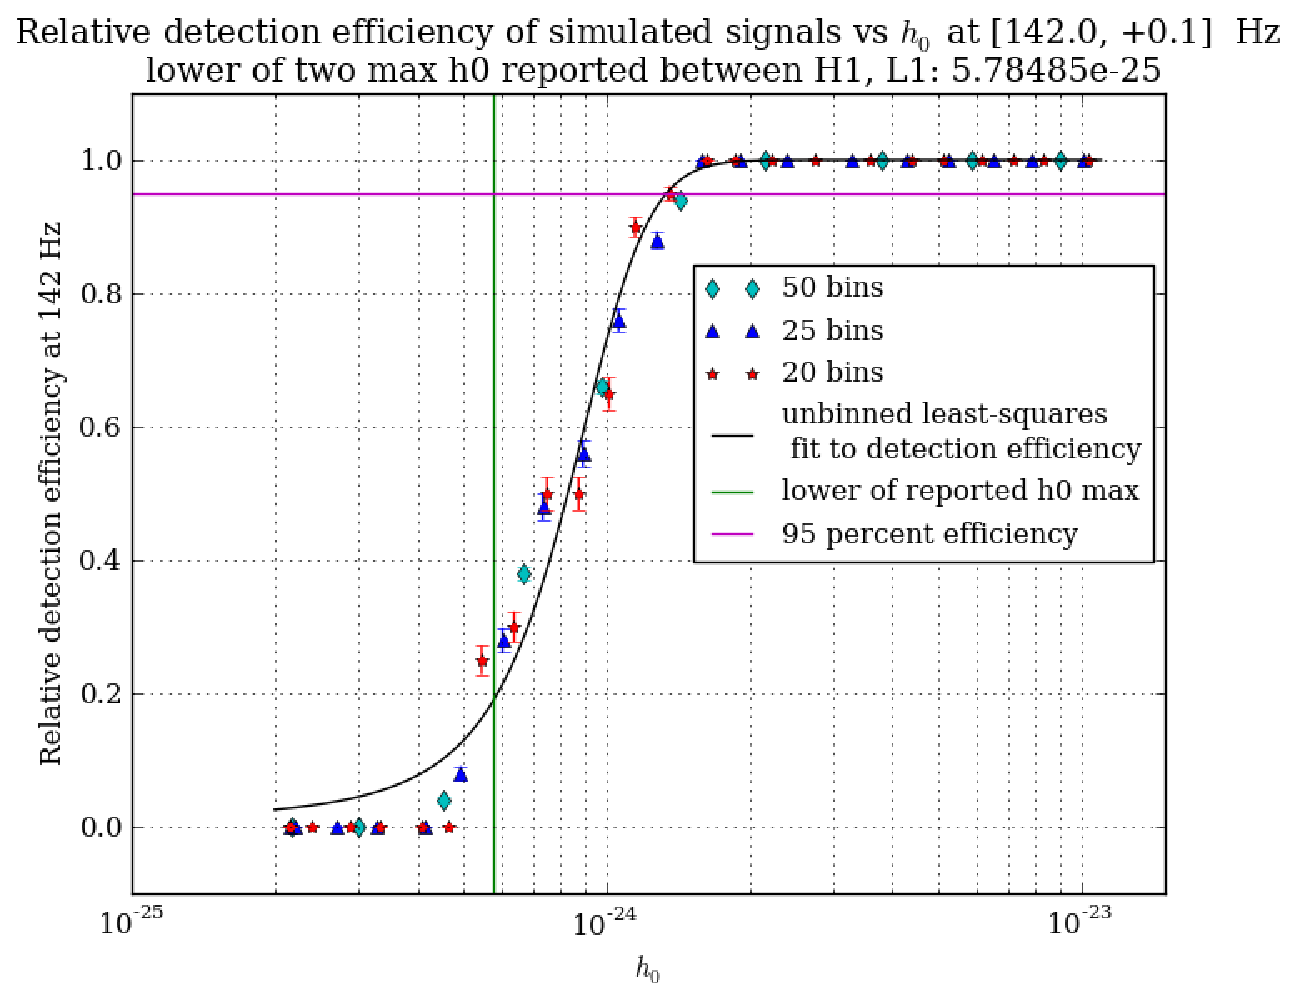
\includegraphics[width=0.70\paperwidth,height=0.48\paperheight]{plots/detectionEfficiencyh0-142-0Hz.eps}
\caption{Detection efficiency of 500 injections (each at H1, L1) into
S6 data at 142 Hz, given threshold $\log_{10}p$ = -7.75.
The least-squares curve fit is to a symmetric sigmoid, which matches the data well at high detection efficiency.
Since the 95\% efficiency region is the most interesting, the relatively poor fit at low efficiency is not much concern, although the fit could be improved with additional parameters.}
\label{S6_det_eff_142}
\end{center}
\end{figure}

Figure~\ref{S6_det_eff_142} plots the \textit{detection efficiency} of TwoSpect in a 0.1 Hz test band starting at 142 Hz.
Five hundred signals are injected, with the same astrophysical parameters, into each LIGO interferometer (H1 and L1), with correspondingly different antenna pattern and detector responses.
A separate TwoSpect analysis was run for each injection simulation to avoid cross-contamination.
The results of corresponding analyses were compared between IFOs.
Templates meeting the detection criteria of the Mock Data Challenge (as discussed in Chapter~\ref{chap5}, having a single-template $\log_{10} p \leq -7.75$) were, if coincident in both interferometers by being in adjacent $df$, $f$ pixels, counted as detections.

Every injected signal had some amplitude $h_0$, but we expect the weakest injections to be swamped by detector noise.
Detection efficiency curves illustrate when the signal becomes detectable, a certain fraction of the time, as injection amplitude is varied.
Some signal parameters vary as well, such as polarization (via astrophysical $\cos \iota$ and $\psi$), frequency and $a \sin i$, and in-band differences in the noise realization make the same $h_0$ detectable or not, depending on these nuisance parameters.
The detection efficiency curve is marginalized, that is, ignores these extra parameters to show only detection rate vs $h_0$.
TwoSpect begins to detect roughly 95\% of injections when $h_0$ is about 10\% of the strain amplitude spectral density (in $1/\sqrt{\textup{Hz}}$) of the detector.

        \subsection{Real S6 data: $h_0$ recovered vs injected}

\begin{figure}
\begin{center}
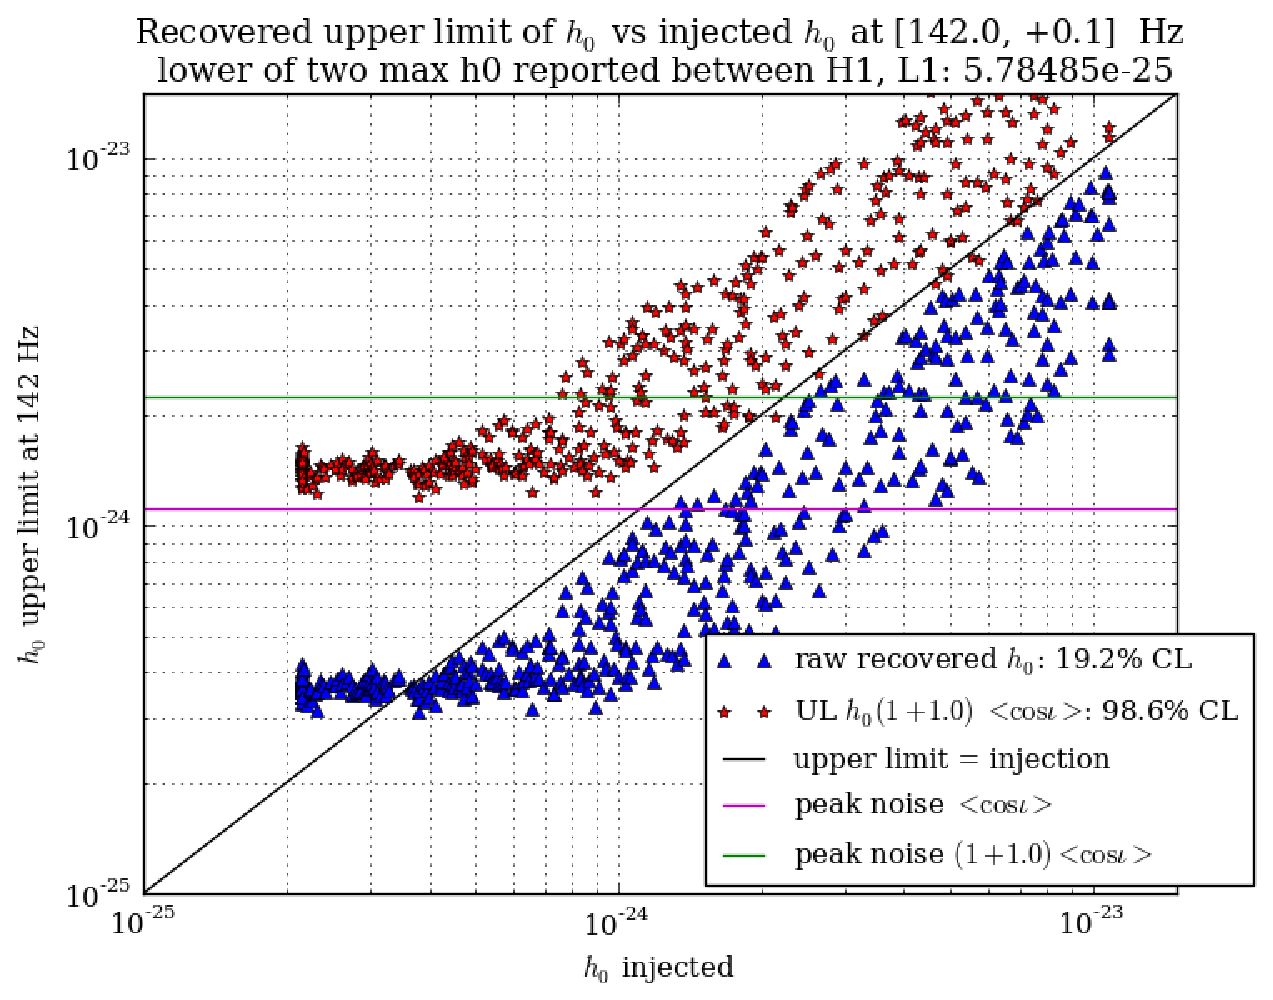
\includegraphics[width=0.70\paperwidth,height=0.48\paperheight]{plots/h0UL-vs-h0injected-142-0Hz.eps}
\caption{
Raw $h_0$ \& tentative 95\% confidence UL $>2\times10^{-24}$; 500 injections
into S6 data at 142 Hz (injections also done at 162, 222 Hz)}
\label{S6_ULs_142}
\end{center}
\end{figure}

Using the same set of injections as for detection efficiency, one can also recover estimated $h_0$ values, as Figure~\ref{S6_ULs_142} illustrates.
TwoSpect returns an $h_0$ proportional to $R^{1/4}$, but the proportionality constant was found to be slightly off in the MDC from that used in all-sky searches, prompting an empirical rescaling by 1.11.
Moreover, studies of the $\cos \iota$ uncertainty had led us to correct $h_0$ estimates further when assuming random polarization: a uniform distribution of $\cos \iota$ values near the detection threshold induced a $1.74 \pm 0.37$ factor, so we multiplied the S6 injections by $1.74$.
The real data injections were necessary to clarify how these $h_0$ levels corresponded to a given confidence level. 
In other words, the reported UL should be above the injected $h_0$ at least 95\% of the time.

Figure~\ref{S6_ULs_142} reports the fraction of the total injection set for which our final formula yields a UL greater than the injected $h_0$, which is higher than 95\% because the formula must hold locally over the entire range.
When attention is restricted to $h_0 > 2\times10^{-24}$, we find that the confidence level multiplier must be 2.0.
Assembled, a UL for each 0.1 Hz band is reported by the formula,

\begin{equation}
h_{0,\textup{ UL, band}} = 2.0 \times 1.74 \times 1.11 \times \textup{sup}(\{h_{0, \textup{ reported, band}}\}).
\label{S6_UL_formula}
\end{equation}

\noindent With coincident analysis of interferometers, the lowest UL reported for a band is taken as the joint UL.
This criterion and Equation~\ref{S6_UL_formula} supersede the single MDC UL with a frequency-dependent UL, calculated for each 0.1 Hz band between 40 and 2040 Hz.

See Appendix~\ref{appendix2} for more details on injection studies.

%\section{S6: Scorpius X-1}

        \section{Scorpius X-1 search using Directed TwoSpect in S6}
        \label{directed_results}
 
            %Preliminary results of a directed search (possibly simulation-only).

            %We have a great deal of material here already, just need to pull from figures and commentary from the Sco X-1 wiki. Keith recommends paralleling the Sco X-1 paper.



\subsection{S6: Scorpius X-1 search plan}

Studies completed, the author has conducted a 2 kHz, $\pm 3 \sigma_{a \sin i}$ search over all S6 data from H1 \& L1.
Stated again briefly, we analyzed the following:
\begin{itemize}
\item 40 to 360 Hz with 840-s SFTs,
\item 360 to 2040 Hz with 360-s SFTs,
\item Overlapping band verifying 260 to 360 Hz with 360-s SFTs,
\item Overlapping band verifying 1400 to 2040 Hz with 300-s SFTs
%\item Search over 300+1100 Hz = 1.4 kHz complete on H1
%\item Search over 300+1700 Hz = 2.0 kHz complete on L1
\end{itemize}
As of this writing, the first three items are complete and the fourth well under way.
The similarity in results between primary (840-s SFT) and overlapping (360-s SFT) bands between 260 and 360 Hz suggests that the high frequency overlap will also yield concordant results.
Thus the author derives ULs for 40 to 360 Hz from the 840-s SFTs and 360 to 2040 Hz from the 360-s SFTs, as described below.

\subsection{S6: Scorpius X-1 heatmaps}

\begin{figure}
\begin{center}
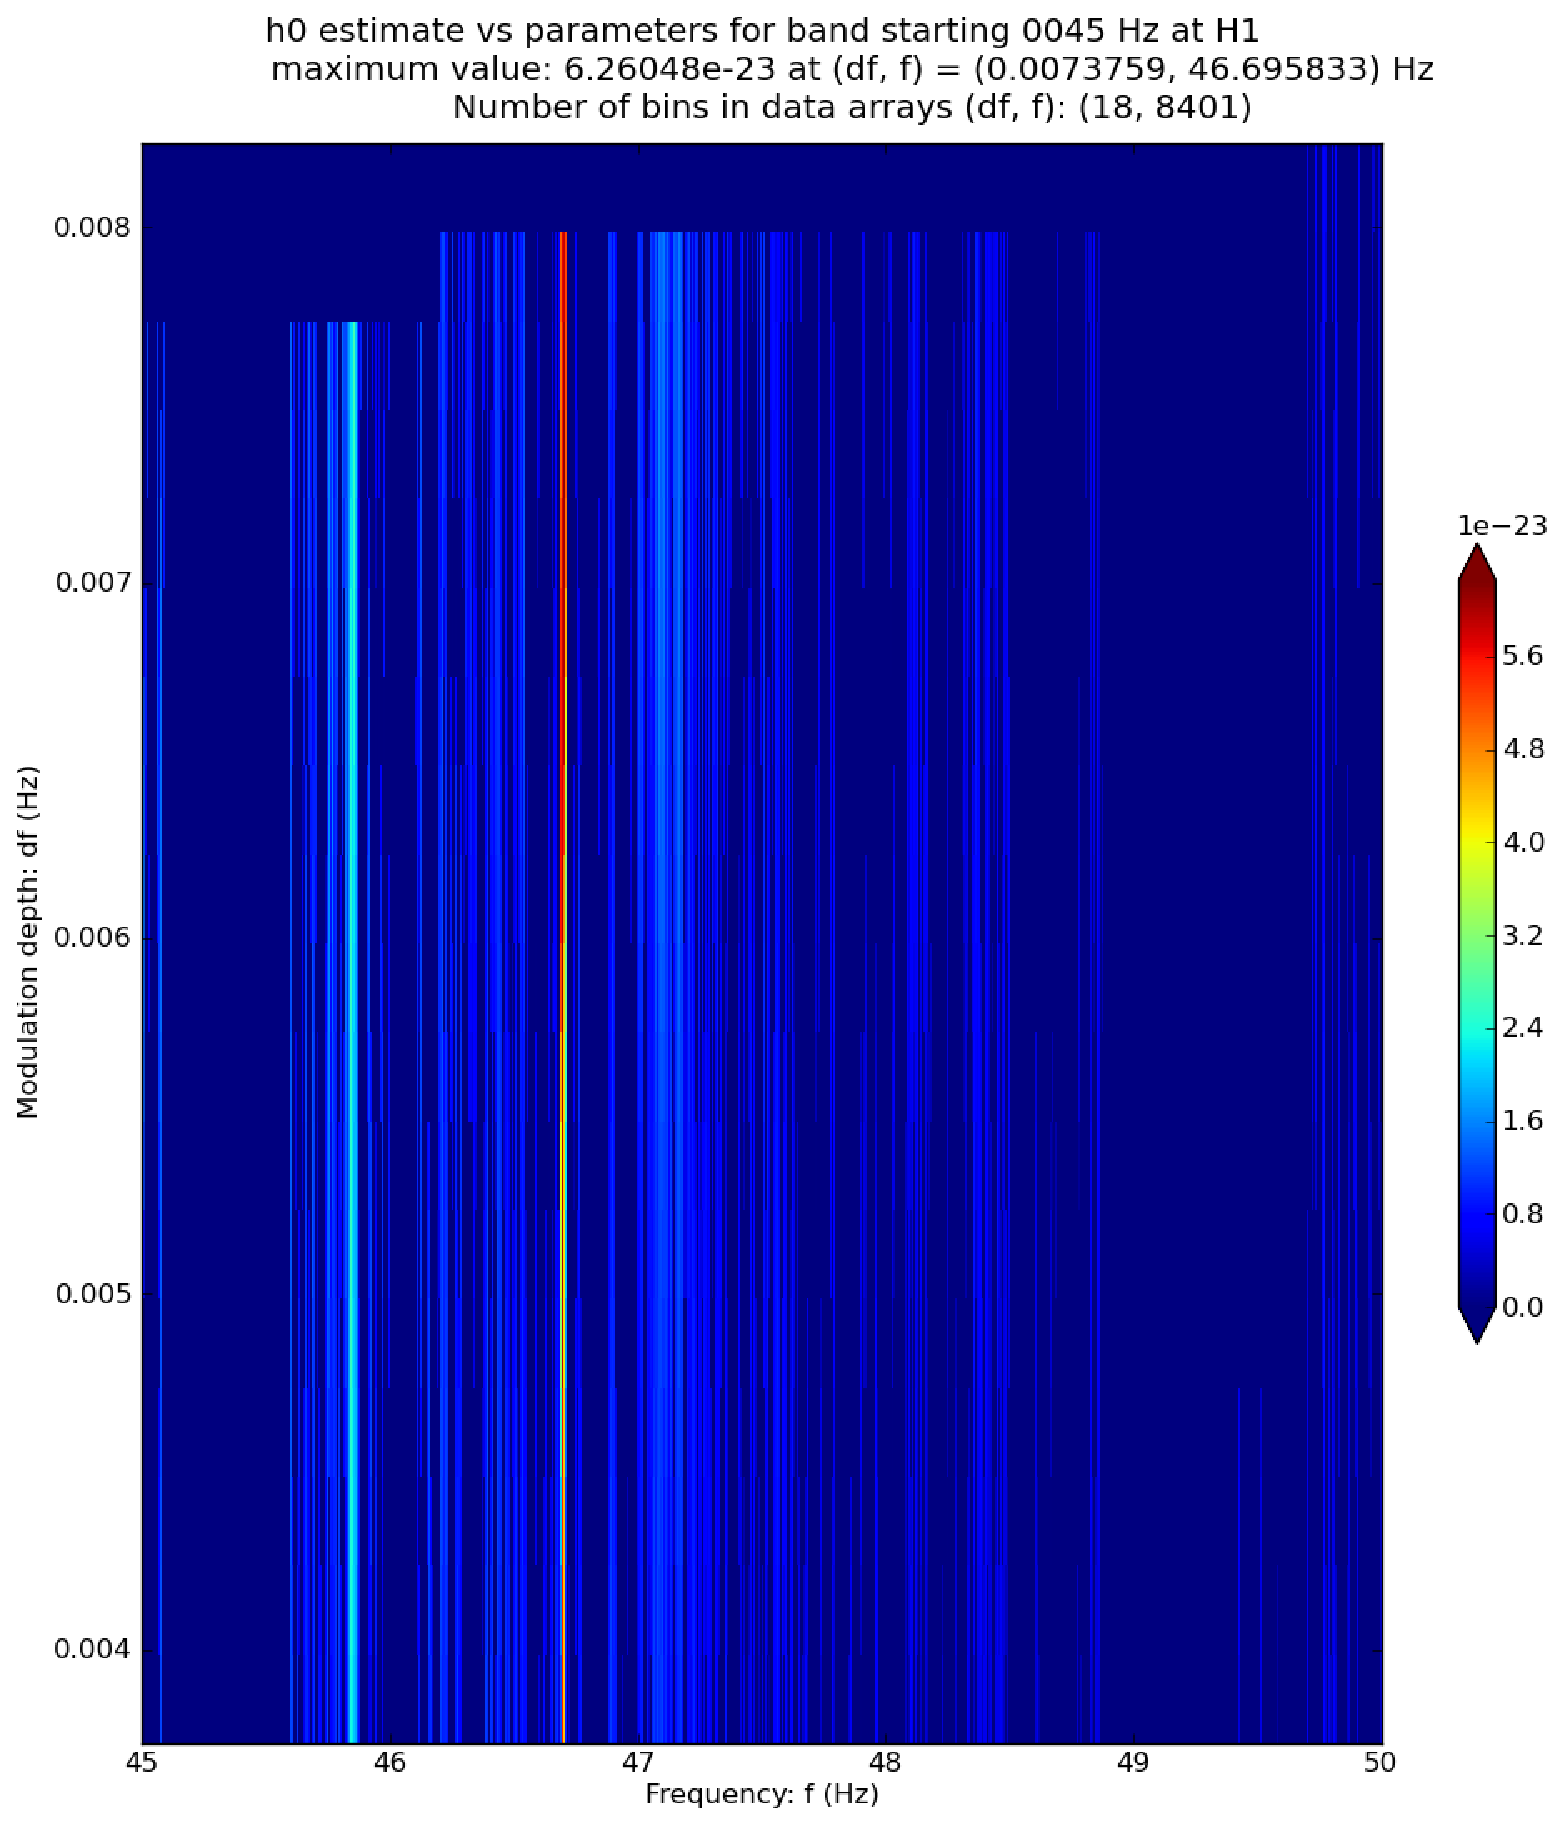
\includegraphics[width=0.68\paperwidth,height=0.48\paperheight]{plots/DFvsFresultsh0-H1_pulsar-0045.eps}
\caption{
S6 $h_0$ heatmap shows real data features, such as 46.7 Hz cal line}
\label{S6_cal_line_heatmap}
\end{center}
\end{figure}

As the S6 search was run on the Atlas cluster at AEI Hannover, individual bands could be checked for consistency with known artifacts.
Heatmaps plotting the intensity of $R$, $\log_{10}p$ and estimated $h_0$ (as reported, not corrected by Equation~\ref{S6_UL_formula}) were generated.
Figure~\ref{S6_cal_line_heatmap} shows one set of 50 bands, spanning 5 Hz, on H1.
This band clearly shows the presence of the 46.7 Hz \textit{calibration line}\footnote{These lines help calibrate the $h_0$ amplitude spectral density~\cite{MeadorsFeedforward2014}, although their TwoSpect reported amplitude may not match the intended $h_0$ because the lines are not modulated like neutron stars in binary systems.}.
Seeing known spectral features at their expected frequencies confirms that TwoSpect is reading data accurately. 
The heatmaps can also be used to follow-up on interesting outliers.

\subsection{S6: Scorpius X-1 upper limits, random polarization}

\begin{figure}
\begin{center}
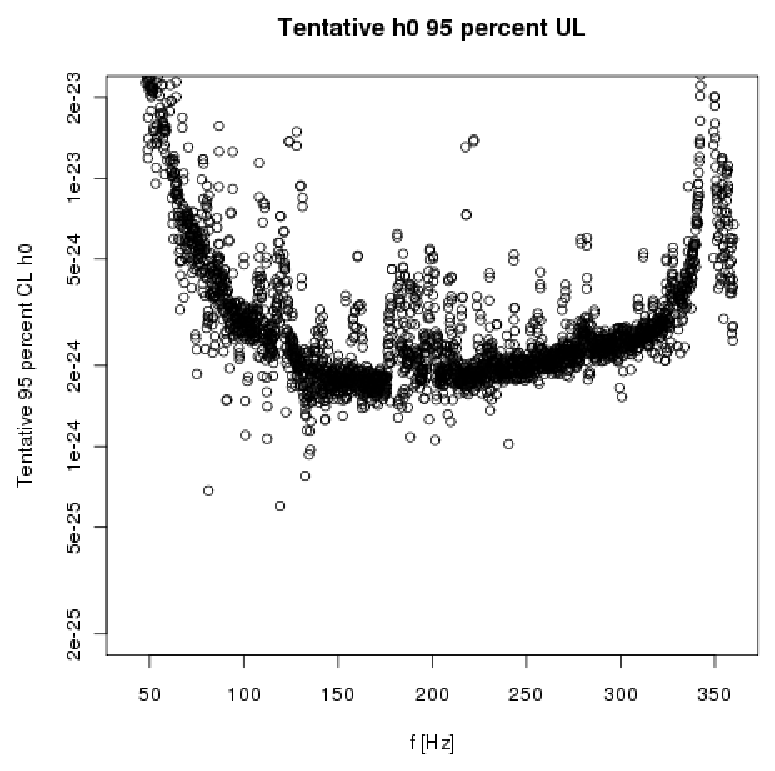
\includegraphics[width=0.68\paperwidth,height=0.48\paperheight]{plots/h0FullUL95logGuess-H1.eps}
\caption{
H1: loudest $h_0 \times \left( 1 + 0.8 \right) \times \left[\cos \iota \textup{ factor}\right]$ in 0.1 Hz bands. This formula corresponds to about 90\% confidence in random polarization ULs in the final analysis.}
\label{S6_H1_UL}
\end{center}
\end{figure}

\begin{figure}
\begin{center}
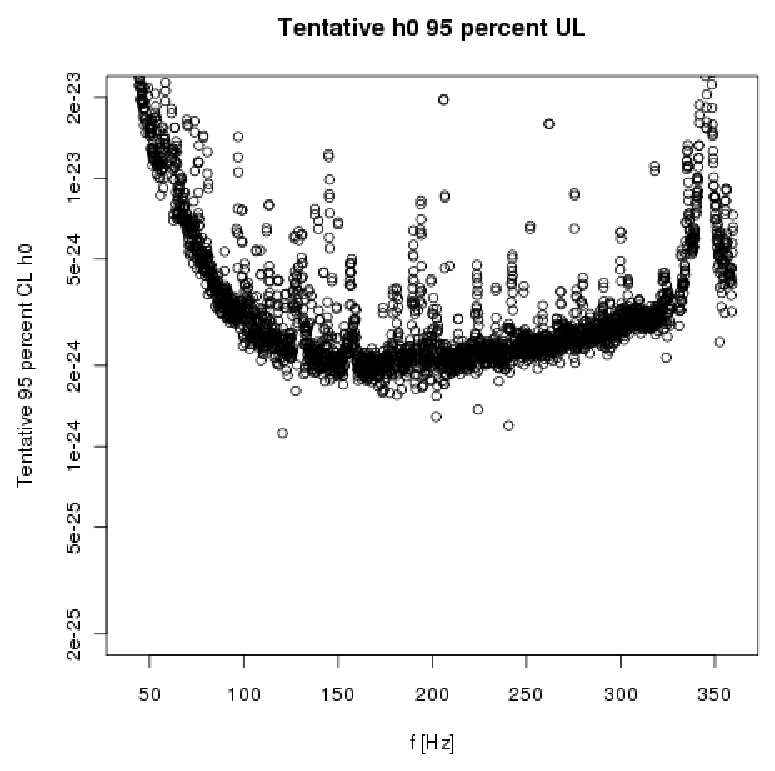
\includegraphics[width=0.68\paperwidth,height=0.48\paperheight]{plots/h0FullUL95logGuess-L1.eps}
\caption{
L1: loudest $h_0 \times \left( 1 + 0.8 \right) \times \left[\cos \iota \textup{ factor}\right]$ in 0.1 Hz bands. This formula corresponds to about 90\% confidence in random polarization ULs in the final analysis.}
\label{S6_L1_UL}
\end{center}
\end{figure}

\begin{figure}
\begin{center}
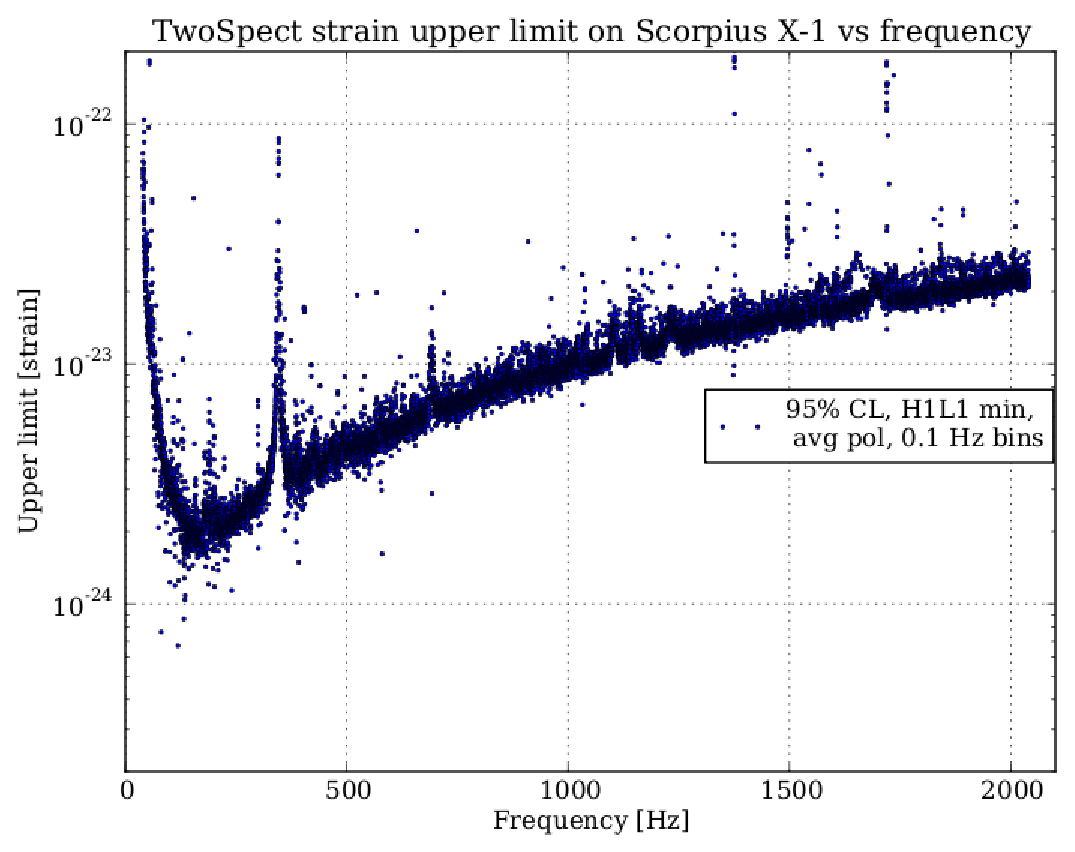
\includegraphics[width=0.68\paperwidth,height=0.48\paperheight]{plots/ScoX1ULs.eps}
\caption{
Joint upper limits for Scorpius X-1, using a confidence interval given by reported $h_0 \times \left( 1 + 1.0 \right) \times \left[\cos\iota \textup{ factor}\right]$ in 0.1 Hz bands. 
This spectrum covers 40 to 2040 Hz using the lower upper limit from either interferomer (H1 or L1) when both yielded data. 
A total of 28.8 Hz were in bands that yielded no real upper limit (because the quarter root of the test statistic was imaginary) in either interferometer, generally due to excessive noise in that band.
Bands were left-closed and right open, e.g., $\left[ 40.0,40.1\right), \left[ 40.1,40.2\right)\ldots \left[2039.9,2040.0\right)$.
}
\label{S6_H1L1_UL}
\end{center}
\end{figure}

Most important are the upper limits (ULs).
TwoSpect has been configured to analyze only `usable SFTs', which must pass a Kuiper's test.
Non-Gaussian or otherwise extremely noisy data is not used.
The 60 Hz and first three harmonic lines (120, 180, 240) Hz harmonic lines, as well as frequencies near the violin modes around 330 Hz, are excluded by these tests.
Altogether, the 40 to 360 Hz H1 search excluded 16.4 Hz and L1 16.2 Hz, while the 360 to 2040 Hz H1 search excluded 21.4 Hz and L1 16.9 Hz of search bands.
For generating upper limits, only 28.8 out of 2000.0 Hz could not be determined from either interferometer.

Figures~\ref{S6_H1_UL} and~\ref{S6_L1_UL} show tentative ULs that, in the final analysis, correspond to approximately 90\% confidence for random polarization.
These figures also illustrate the most sensitive part of the LIGO spectrum.
The entire spectrum, with the final 95\% confidence UL for random polarization, is shown in Figure~\ref{S6_H1L1_UL}.

Previous Radiometer surveys using S5 data~\cite{AbadieStoch2011} may appear to show a better, lower UL, but the results are not directly comparable.
The Radiometer UL is calculated for 90\% and is for circular (optimal) rather than random, polarization.
In addition, signal leakage across the 0.25 Hz bins used in the Radiometer search leads to UL degradation by as much as 70\% at a frequency of 1500 Hz\footnote{Confirmed in private communication and will be noted in the forthcoming Bulten \textit{et al} Sco X-1 paper~\cite{ScoX1MDC2014DCC}.}.
TwoSpect's S6 UL is competitive (possibly better, pending deeper understanding of the algorithmic differences).
Moreover, given an outlier, TwoSpect could do something not yet possible with other comparable pipelines: measure the projected semimajor axis, $a \sin i$.

\subsection{S6: Scorpius X-1 outliers}

\begin{table}
\begin{center}
\begin{tabular}{r r l}
Outlier Number & Frequency (Hz) & Explanation \\
\hline
1 & 42.00 & -- \\
2 & 64.00 & Power of 2 line \\
3 & 108.10 & -- \\
4 & 108.85 & -- \\
5 & 109.50 & -- \\
6 & 111.02 & -- \\
7 & 128.00 & Power of 2 line \\
8 & 139.52 & -- \\
9 & 154.04 & -- \\
10 & 156.82 & -- \\
11 & 157.99 & -- \\
12 & 158.36 & -- \\
13 & 158.87 & -- \\
14 & 190.86 & -- \\
15 & 192.54 & Injected pulsar 8? \\
16 & 200.53 & -- \\
17 & 200.60 & -- \\
18 & 209.21 & -- \\
19 & 209.28 & -- \\
20 & 223.66 & -- \\
21 & 256.02 & Power of 2 line \\
22 & 268.13 & -- \\
\end{tabular}
\caption{List of Scorpius X-1 outliers in the search of S6 data. This list covers 40 to 360 Hz.}
\label{ScoX1S6outlierTable}
\end{center}
\end{table}

Table~\ref{ScoX1S6outlierTable} presents a list of outliers present in both intereferometers between 40 and 360 Hz.
Analysis of outliers from 360 to 2040 Hz is forthcoming.
Some coincident outliers present in the initial analysis include lines at powers of 2 and a probable trace of a hardware-injected simulated pulsar.
As noted earlier, power line frequencies and violin modes were automatically dismissed by TwoSpect because.
More exhaustive study of the candidates in Table~\ref{ScoX1S6outlierTable} will continue, although GW detection would be a rather too-optimistic prospect given the torque-balance limit for Scorpius X-1~\cite{Bildsten1998} and estimated detection efficiency.

The search for GW from Scorpius X-1 continues, and the imminent observational runs of aLIGO give hope that its signature may soon be detected.
With continued improvements to CW algorithms and the enhanced sensitivity of future interferometers, we expect that Giacconi's discovery of the first and brightest extrasolar X-ray source will be paralleled with a GW discovery.

\section{XTE J1751-305 search using Directed TwoSpect in S6}

\subsection{S6: XTE J1751-305 background}

Discovered by Markwardt \textit{et al} in 2002~\cite{Markwardt2002}, the X-ray transient (XTE) J1751-305 has indications it too could emit GW~\cite{Strohmayer2014}.
As detailed by Strohmayer and Mahmoodifar, J1751 has been searched for signs of non-radial oscillation modes, such as $r$- (and $g$-) modes.
No $r$-modes have so far been seen.
Preliminary results suggested that $r$-modes might be consistent with X-ray observations.
Subsequently, Andersson \textit{et al}~\cite{Andersson2014} argued that an $r$-mode would have already spundown below detectable levels, but Lee~\cite{Lee2014} reflected that a crust-only surface $r$-mode might still be present. 
 J1751 is an intriguing candidate in its own right and highlights the different kinds of directed GW search that TwoSpect can conduct.

J1751 is the XTE with the shortest known period,
P $\approx$$ $ 2545.3 seconds or 42 minutes, and $a \sin i$ $\approx0.010\pm0.003$s.
Crucially, its spin frequency, unlike that of Scorpius X-1, is known with microHertz precision: $f = 435.31799$ Hz.
A search can thus be fast ($< 10^5$ templates).
At an estimated $d > 7$ kpc, near the galactic center, J1751 is distant for a CW source, but the chance of a $r$-mode motivates a quick look.
We expect GW emission to be most likely at the following frequencies:
%\\
%$\textup{}$

\begin{itemize}
\item $\nu_\textup{spin}$: 435.31799 Hz
\item $r$-mode: (2-0.5727597)*(435.31799 Hz) = 621.3034 Hz
\item $2\nu_\textup{spin}$: 870.63598 Hz
%$\textup{}$
\end{itemize}

%\section{S6: XTE J1751-305}
\subsection{S6: XTE J1751-305 heatmaps}

\begin{figure}
\begin{center}
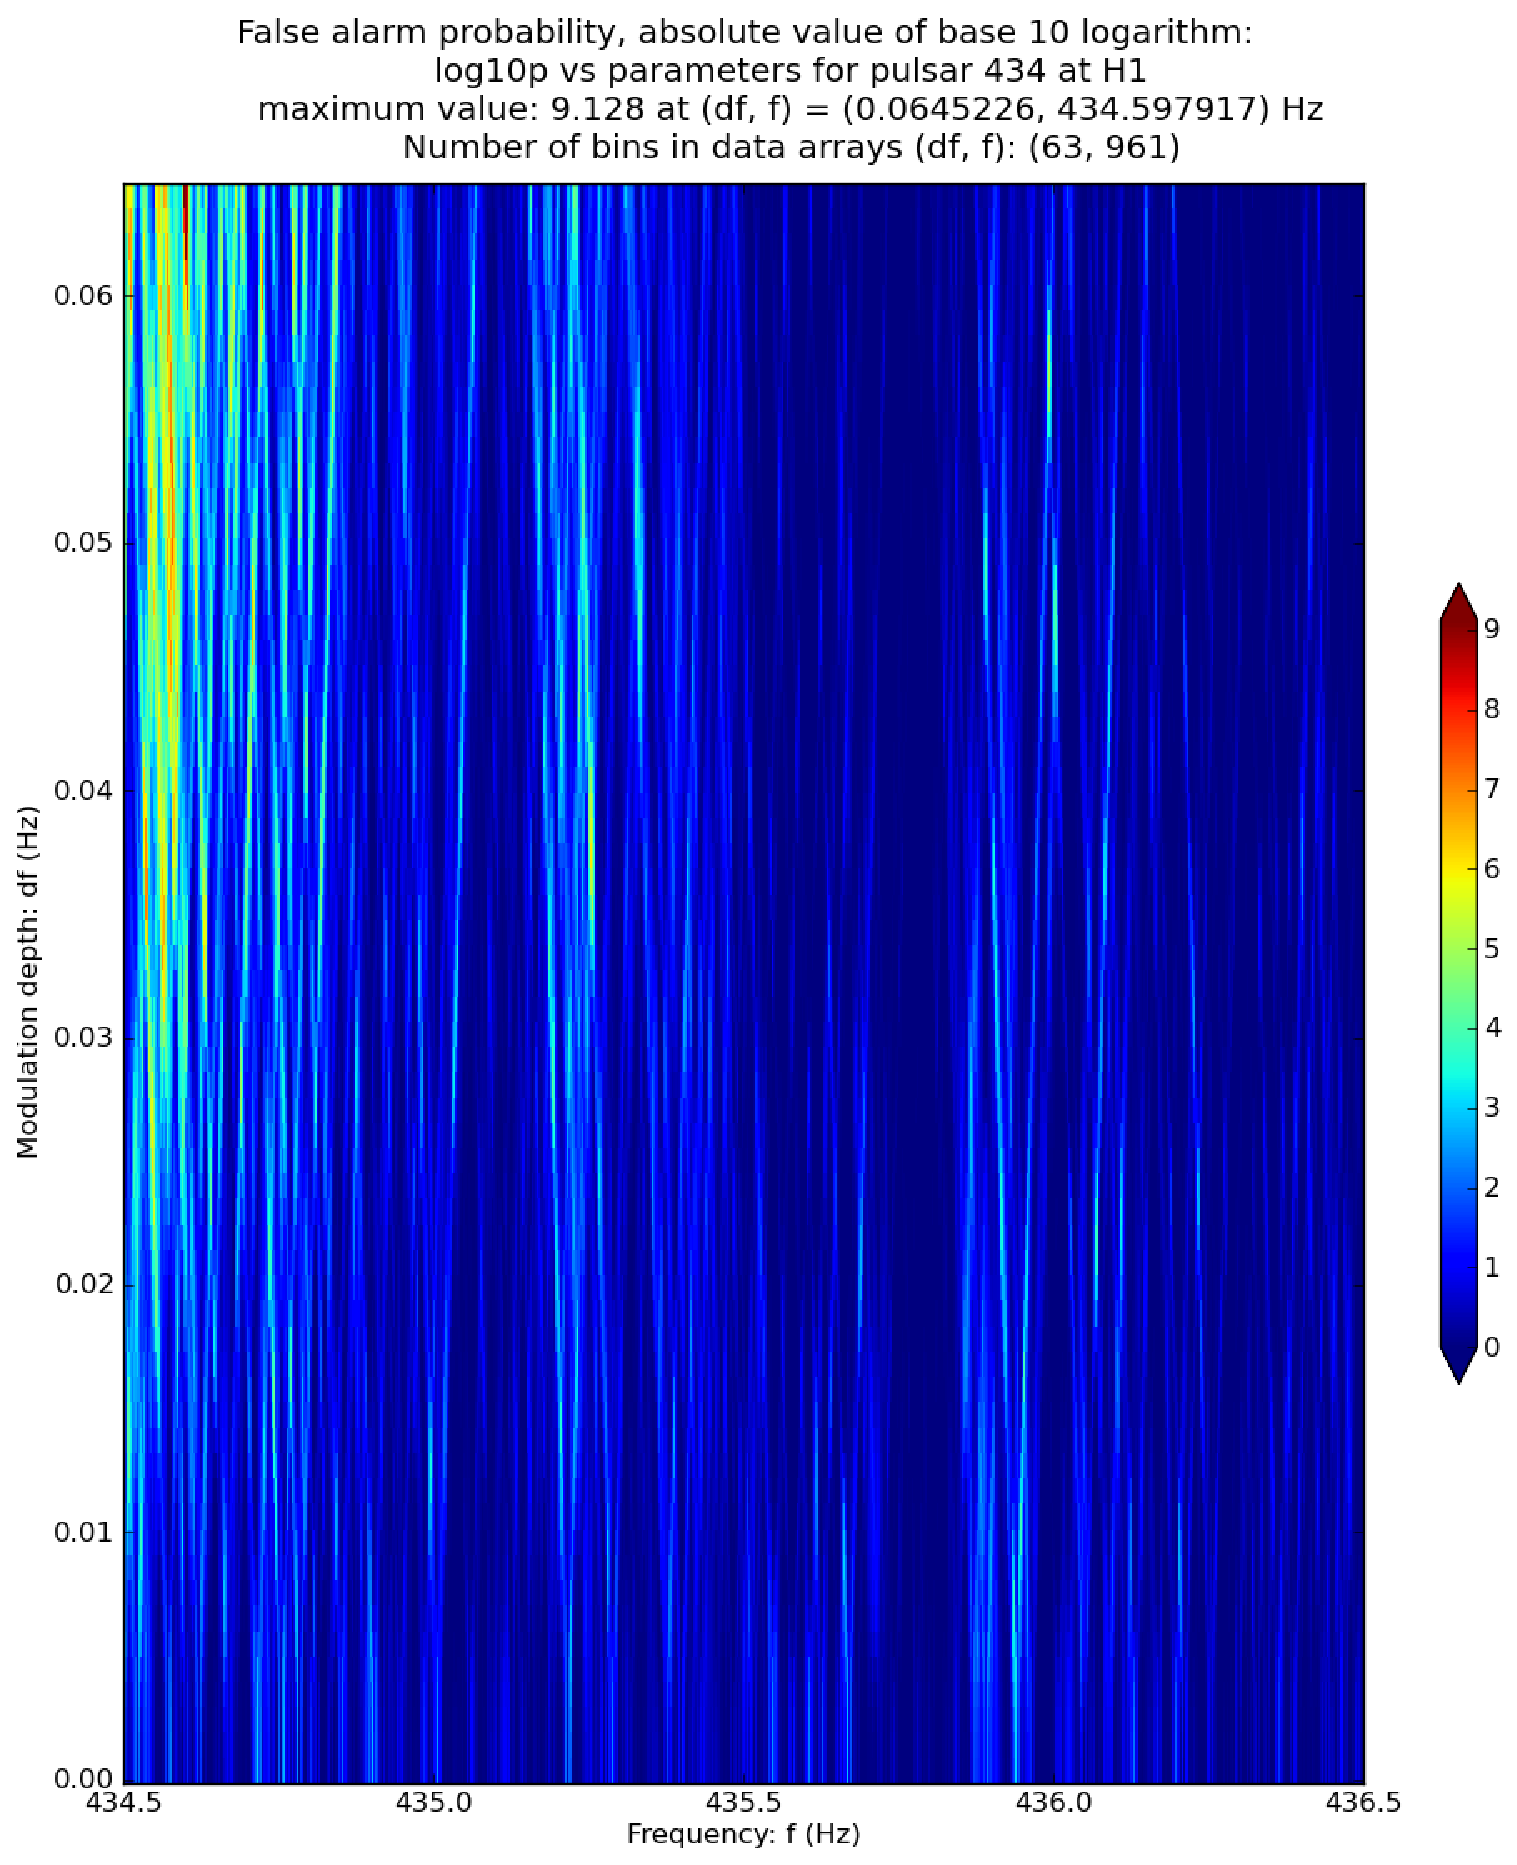
\includegraphics[width=0.68\paperwidth,height=0.48\paperheight]{plots/DFvsFresultsProb-H1_pulsar-434.eps}
\caption{
Quick look at J1751-305, H1 $\log_{10}p$, 435 Hz $\nu_0$}
\end{center}
\end{figure}


\begin{figure}
\begin{center}
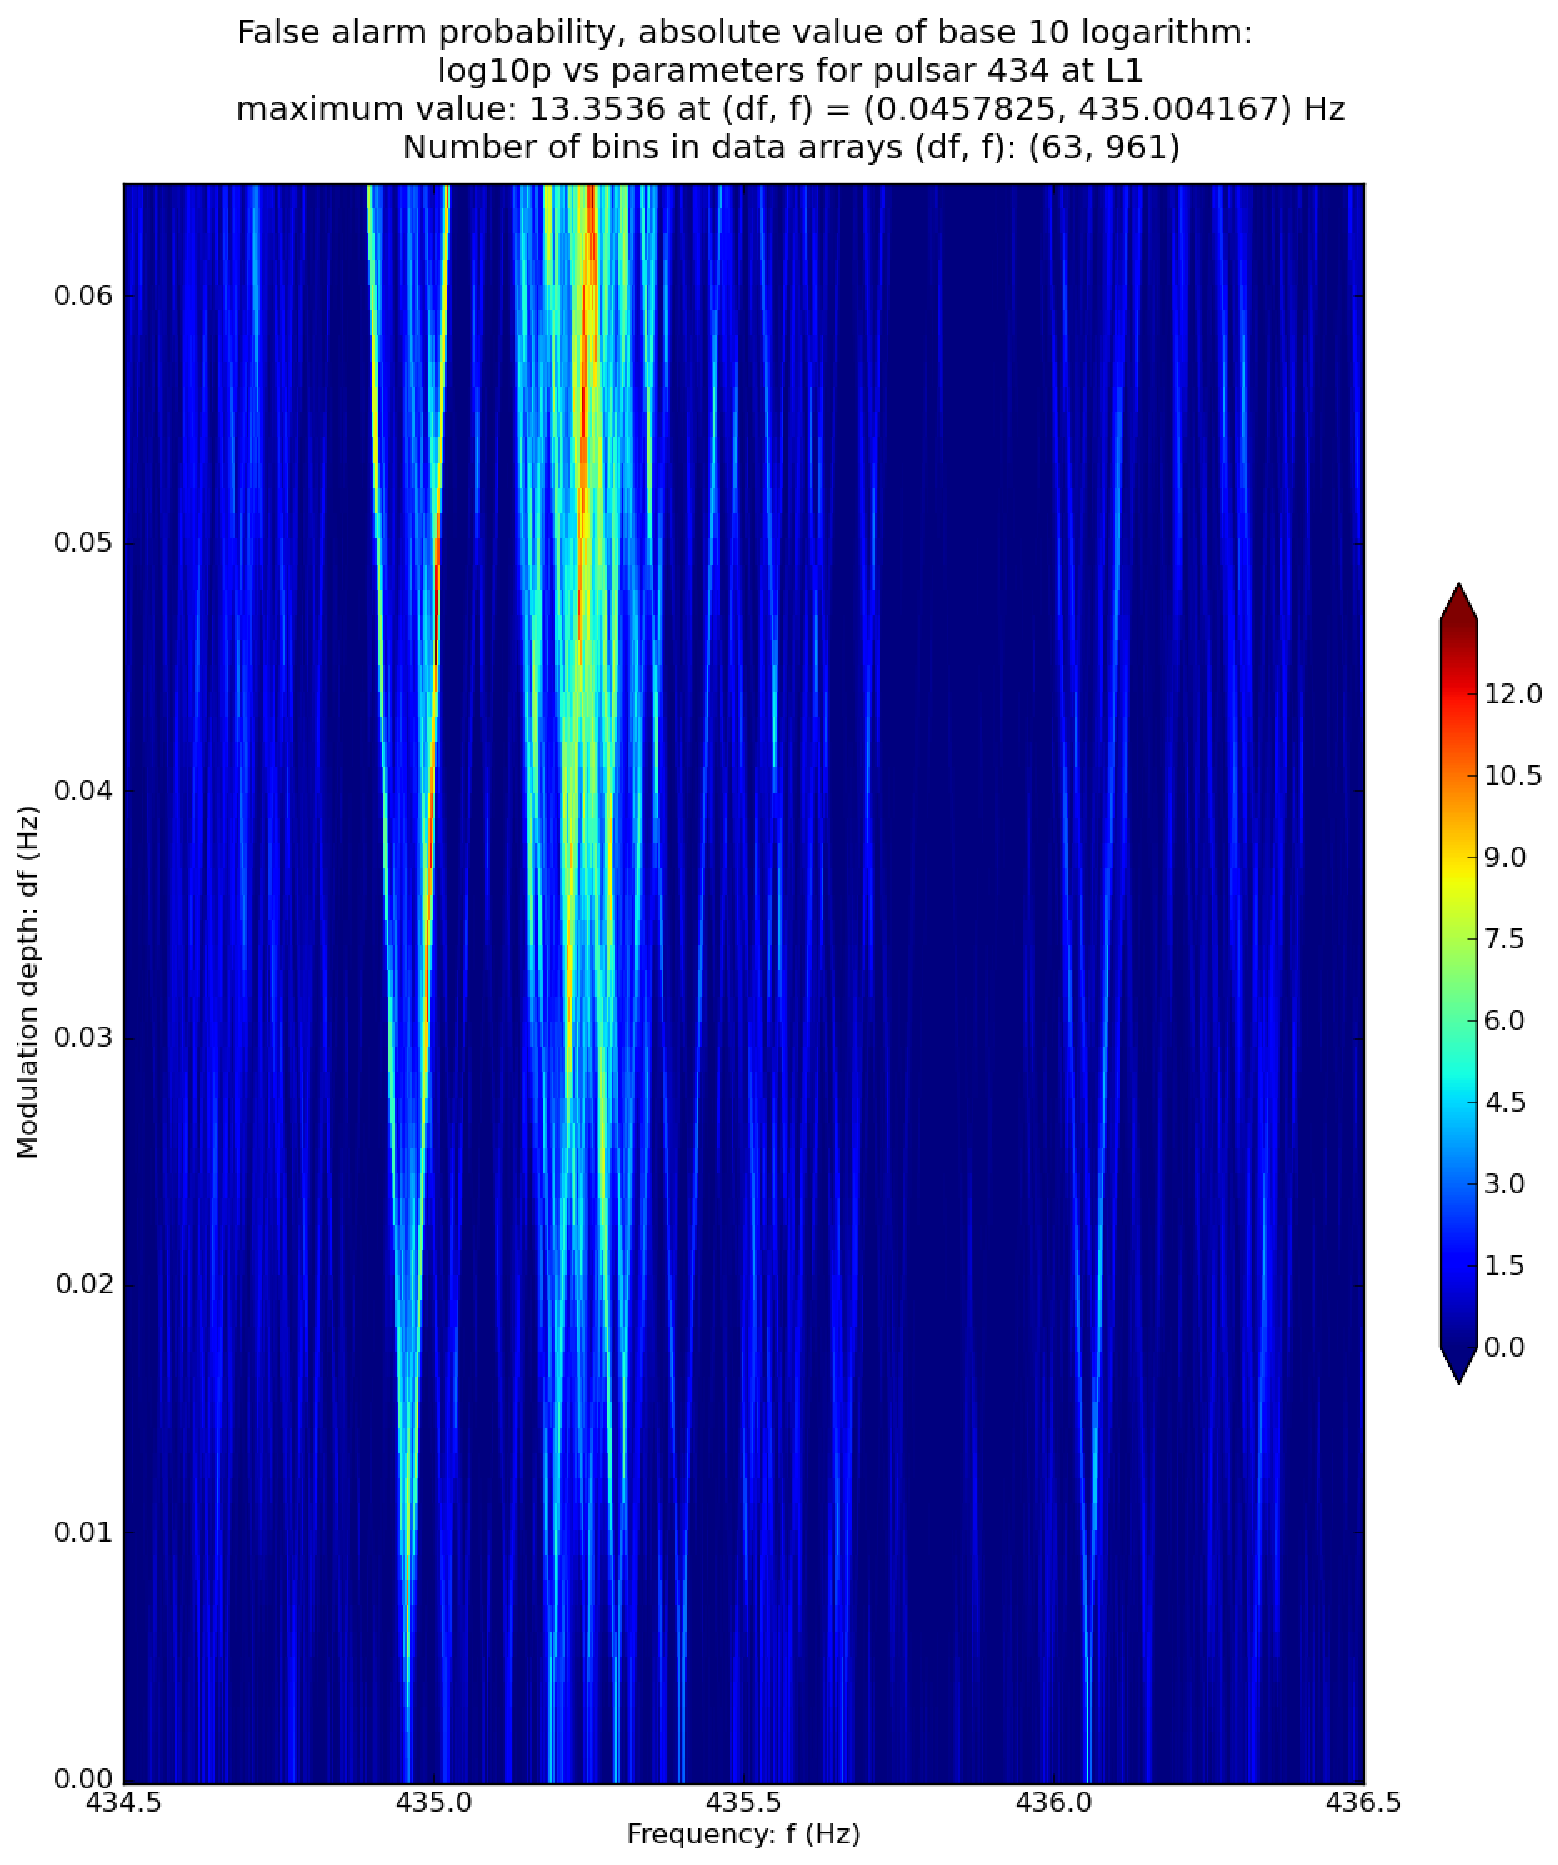
\includegraphics[width=0.68\paperwidth,height=0.48\paperheight]{plots/DFvsFresultsProb-L1_pulsar-434.eps}
\caption{
Quick look at J1751-305, L1 $\log_{10}p$, 435 Hz $\nu_0$}
\end{center}
\end{figure}


\begin{figure}
\begin{center}
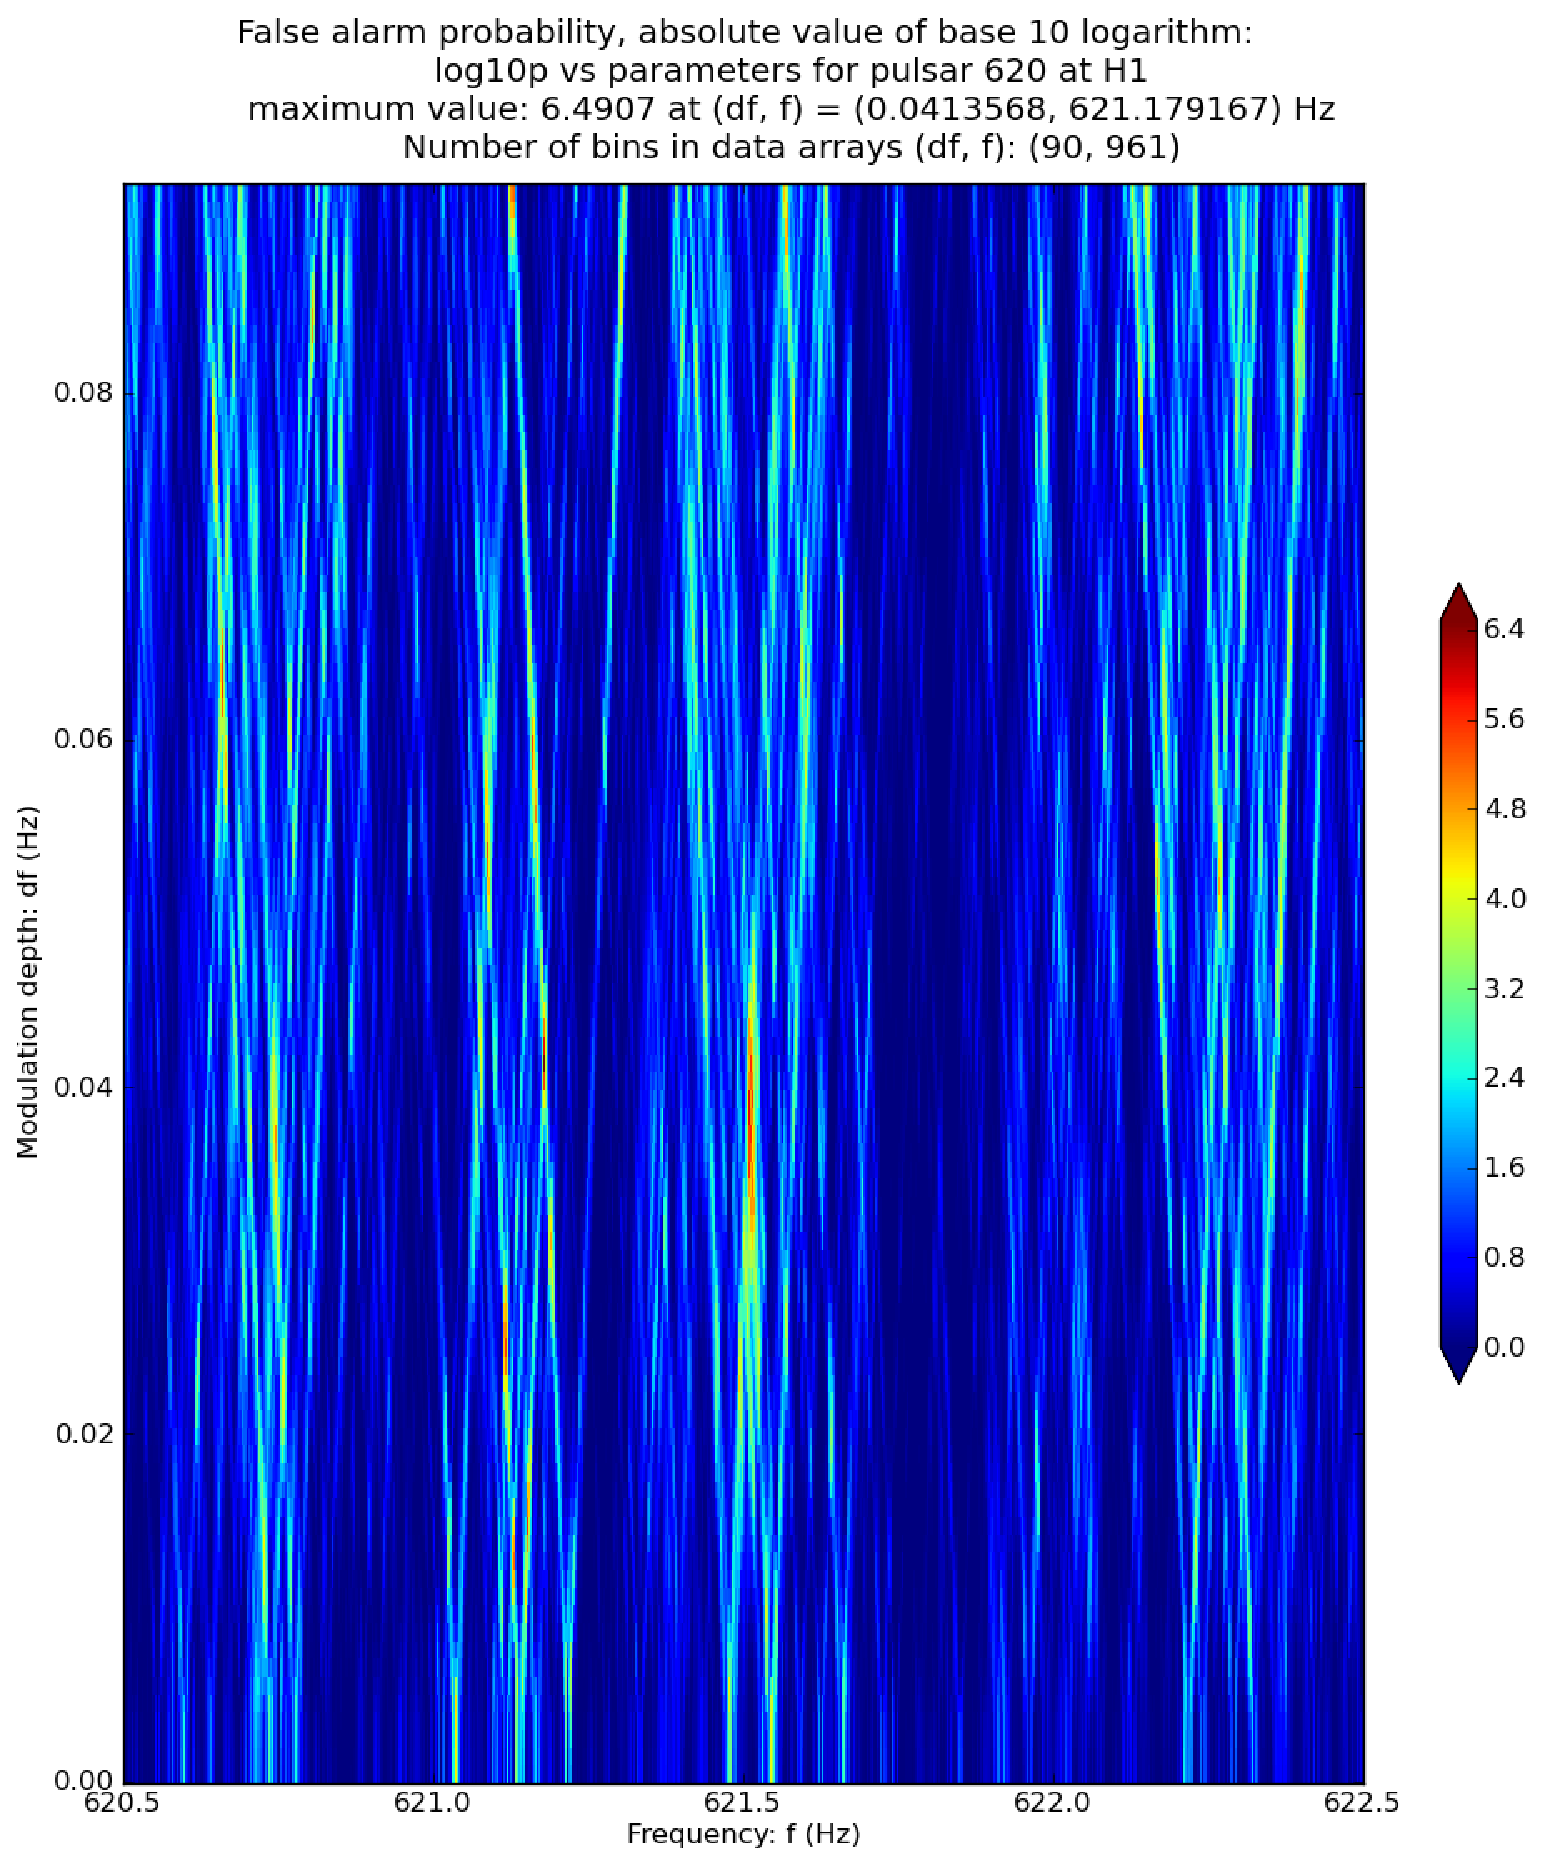
\includegraphics[width=0.68\paperwidth,height=0.48\paperheight]{plots/DFvsFresultsProb-H1_pulsar-620.eps}
\caption{
Quick look at J1751-305, H1 $\log_{10}p$, 621 Hz $r$-mode}
\end{center}
\end{figure}


\begin{figure}
\begin{center}
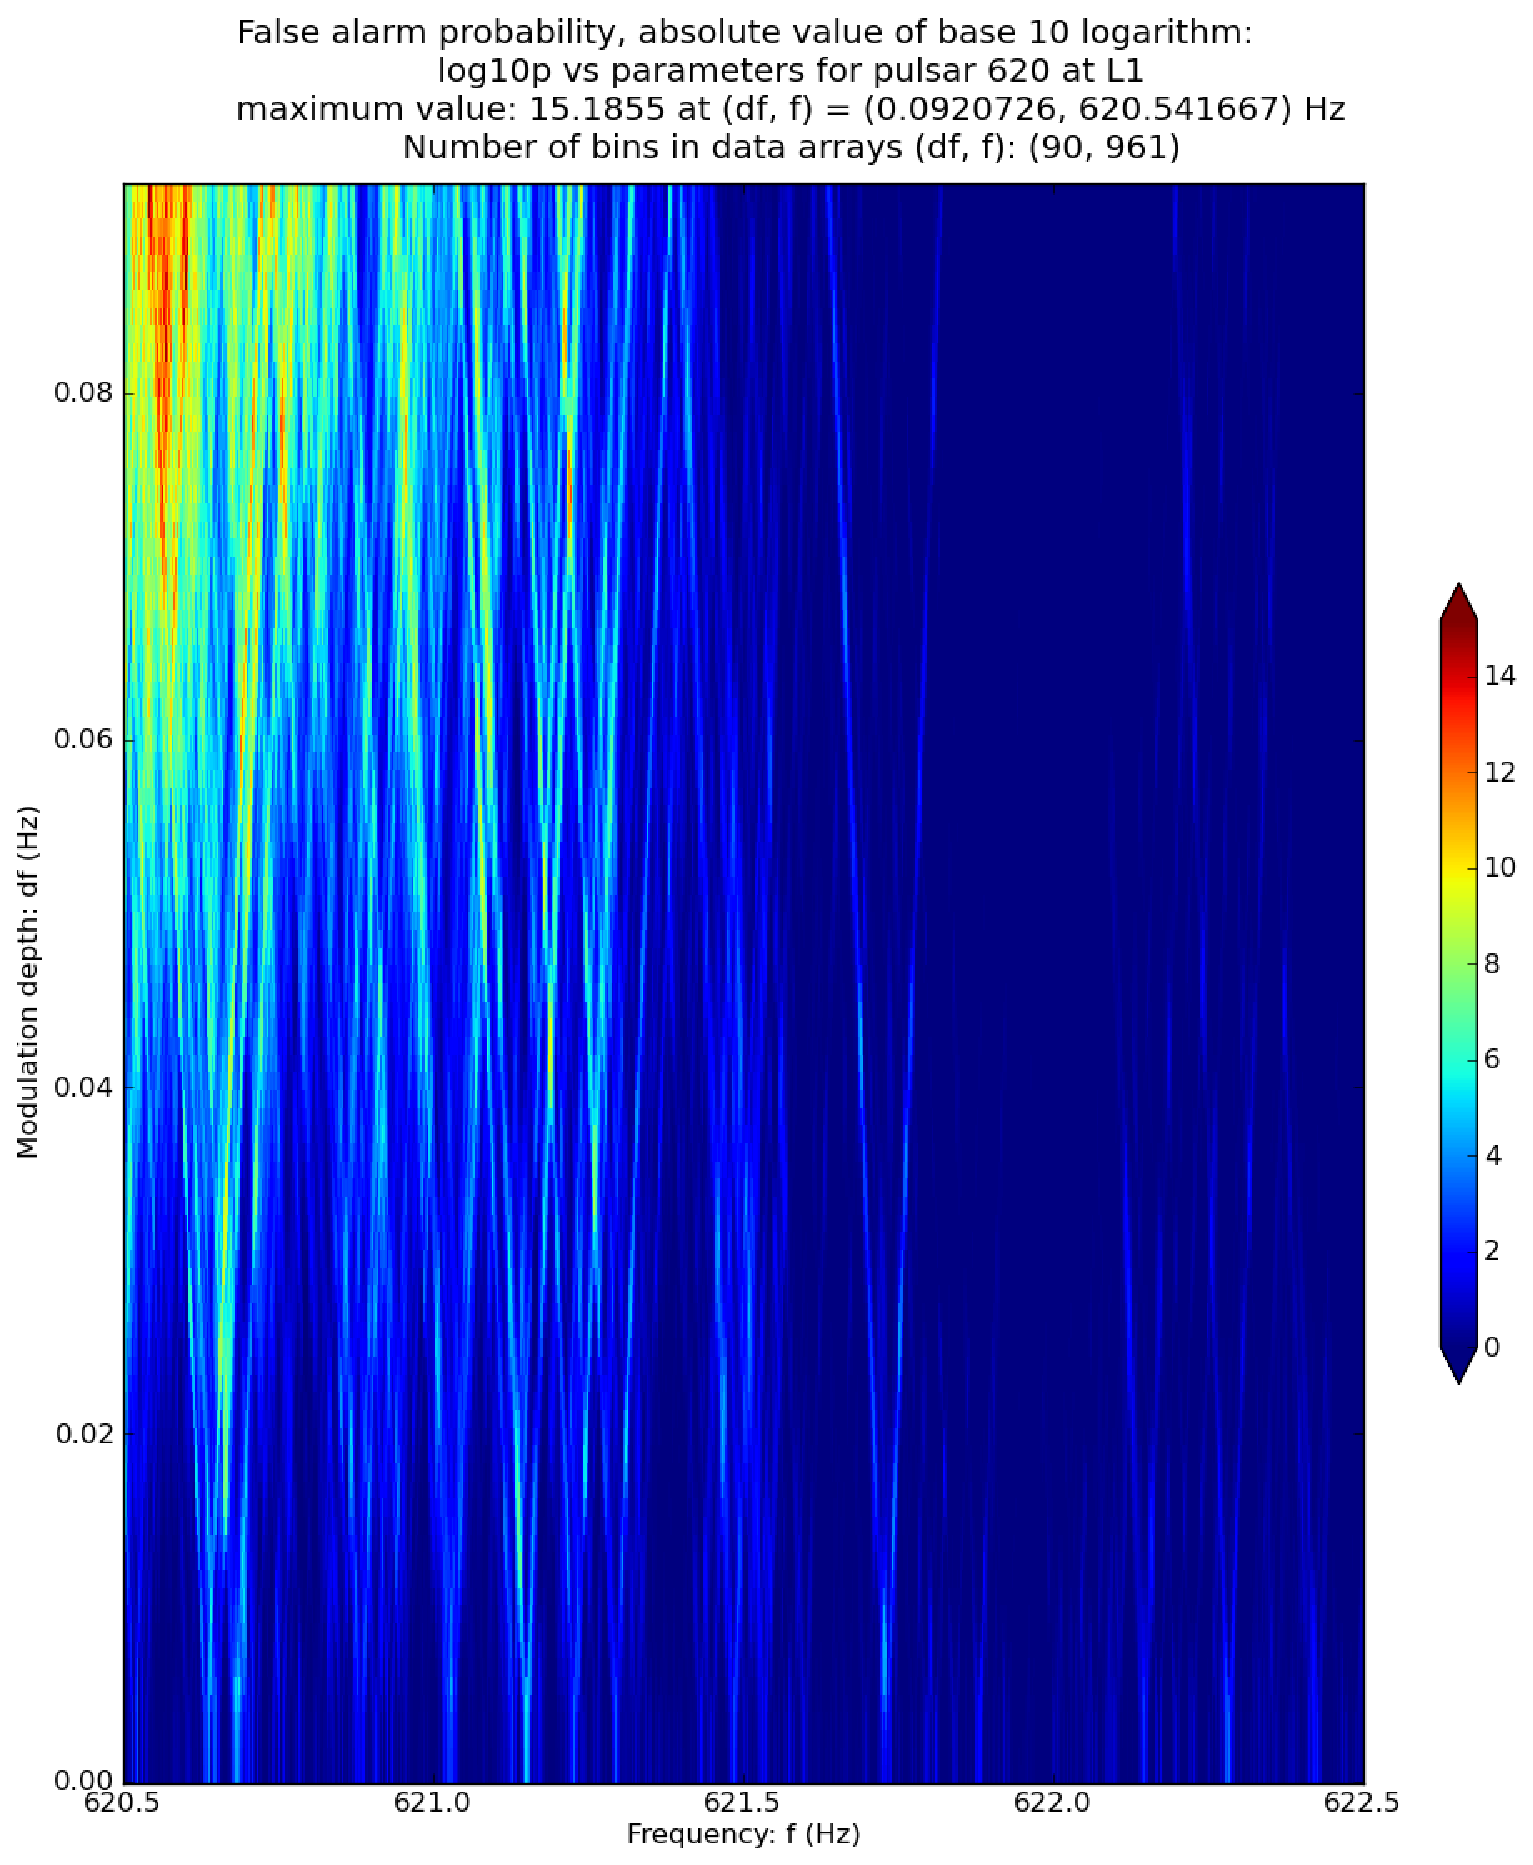
\includegraphics[width=0.68\paperwidth,height=0.48\paperheight]{plots/DFvsFresultsProb-L1_pulsar-620.eps}
\caption{
Quick look at J1751-305, L1 $\log_{10}p$, 621 Hz $r$-mode}
\end{center}
\end{figure}

A straightforward search over $\pm \sigma_{a \sin i}$ is being conducted:

\begin{description}
\item Searched frequencies [434.5,436.5] \& [620.5,622.5] Hz
\item Searching [869.5, 871.5] Hz
\end{description}

A TwoSpect analysis and heatmaps have been made for the $\nu_\textup{spin}$ and $r$-mode bands, and analysis is underway on the $2\nu_\textup{spin}$ frequencies.
Upper limits and candidate comparison can then be made.
Even if no GW signal is seen -- the probable outcome absent $r$-modes -- XTE J1751-305 offers a prototypical search strategy for well-characterized, directed CW sources.


\section{Summary of Directed TwoSpect S6 searches}

The author has conducted a 2 kHz, $\pm 3 \sigma_{a \sin i}$ directed search for Scorpius X-1 over all S6 data from H1 \& L1 using TwoSpect.
The analysis from 40 to 360 Hz used 840-s SFTs,
and from 360 to 2040 Hz used 360-s SFTs,
(to prevent spectral leakage).
This primary analysis (4 kHz of data between the two detectors) has yielded preliminary joint upper limits over the 2 kHz from 40 to 2040 Hz.
Overlapping bands are underway to confirm the results using
360 s SFTs to validate the 260 to 360 Hz band and
300 s SFTs to validate 1400 to 2040 Hz, but initial output justifies treating the existing results as valid. 
%\item Search over 300+1700 Hz = 2.0 kHz complete on H1
%\item Search over 300+1700 Hz = 2.0 kHz complete on L1
%\end{itemize}

Primary analysis for this S6 search was 100\% done in roughly 30 days.
In the process, our post-processing methodology has been adjusted from all-sky techniques~\cite{GoetzTwoSpectResults2014} to one appropriate for a densely-sampled, correlated `$df$ vs $f$' parameter space.
The remaining questions are in the identification of outliers -- already $\sim 22$ coincident features have been noted between 40 and 360 Hz -- and explanation of too quiet bands.
Too quiet bands, seen in Figure~\ref{S6_H1L1_UL}, appear due to the noise subtraction in the $R$ statistic;further investigation will see whether these presumably non-genuine `good' bands can be systematically rectified.

In addition, a search for XTE J1751-305 has been completed, with its own post-processing underway.

%\begin{enumerate}
%\item Should verify overlapping bands with shorter coherence length
%\item Refining upper limit methodology
%\item R statistic: quiet 0.1 Hz bands need investigation
%\item Detection criteria: how applicable is MDC experience?
%\end{enumerate}

%\emph{Random polarization} $h_0$ lower limit might be $< 1.3\times10^{-24}$
%\emph{Outliers} incoming: already $\sim 22$ coincident features in [40, 360] Hz

Scorpius X-1 and XTE J1751-305 are among the best potential sources of GW in the sky.
This chapter shows that we can extract an upper limit around $1.3\times10^{-24}$ from Scorpius X-1 in S6 data and demonstrates that these searches will be practicable in the future.
Advanced LIGO will turn on for O1 in summer 2015: TwoSpect, one of the prime algorithms for finding continuous GW from neutron stars in binary systems, is ready.
%Plans for O1, first aLIGO run

\textit{As previously noted, results from this chapter are preliminary and have not been reviewed yet by the LIGO Scientific Collaboration.}

        %---------------------------------

	%The following is an example of using the commands \textit{ref}
	%and \textit{label}. With these commands theorems, chapters,
	%sections and figurres can be labeld with names in the tex file
	%and then refered to by these names in later tex files. In
	%chapter~\ref{intro} we saw section~\ref{sample_section} or
	%theorem~\ref{sample_theorem}.

	%Lastly, here is how to include a figure. First generate an
	%encapsulated postscript file in xfig, adobe illustrator or
	%some other program. The specific commands are found in
	%\textit{chap2.tex}.

        %\begin{figure}[htb]
        %\centerline{ \epsfig{figure=sample.eps, 
        %height =  1.5 in}}
        %\caption{Sample Figure}
        %\label{sample_figure}
        %\end{figure}

